\documentclass{article}
\usepackage{graphicx}
\usepackage{hyperref}
\usepackage{amsmath}
\usepackage{times}

\textwidth=6.2in
\textheight=8.5in
%\parskip=.3cm
\oddsidemargin=.1in
\evensidemargin=.1in
\headheight=-.3in


%------------------------------------------------------------
% newcommand
%------------------------------------------------------------
\newcommand{\scscst}{\scriptscriptstyle}
\newcommand{\scst}{\scriptstyle}
\newcommand{\Robject}[1]{{\texttt{#1}}}
\newcommand{\Rfunction}[1]{{\texttt{#1}}}
\newcommand{\Rclass}[1]{\textit{#1}}
\newcommand{\Rpackage}[1]{\textit{#1}}
\newcommand{\Rexpression}[1]{\texttt{#1}}
\newcommand{\Rmethod}[1]{{\texttt{#1}}}
\newcommand{\Rfunarg}[1]{{\texttt{#1}}}

\usepackage{Sweave}
\begin{document}
\Sconcordance{concordance:results_zoonotic.tex:results_zoonotic.Rnw:%
1 27 1 1 0 18 1 1 6 1 1 34 0 1 5 5 1 31 0 1 5 1 1 1 21 1 2 4 1 1 53 1 2 %
7 1 1 5 1 2 1 0 1 1 9 0 1 1 19 0 1 2 1 1 1 6 1 2 4 1 1 6 1 2 4 1}


%------------------------------------------------------------
\title{Zoonotic cryptosporidium}
%------------------------------------------------------------
\author{David Hayman}
%\date{}




\maketitle
%\tableofcontents

%-------------------------------------------
\section{Zoonotic - all data}
%--------------------------------------------


\begin{Schunk}
\begin{Sinput}
> fit <- manova(cbind(Species, Gene, Pi, Theta) ~ Zoonotic, data = Pi_data)
> summary(fit, test = "Pillai")
\end{Sinput}
\begin{Soutput}
          Df Pillai approx F num Df den Df Pr(>F)
Zoonotic   1 0.1905   1.4709      4     25 0.2409
Residuals 28                                     
\end{Soutput}
\begin{Sinput}
> summary.aov(fit)
\end{Sinput}
\begin{Soutput}
 Response Species :
            Df Sum Sq Mean Sq F value Pr(>F)
Zoonotic     1  0.025  0.0254  0.0124  0.912
Residuals   28 57.175  2.0419               

 Response Gene :
            Df  Sum Sq Mean Sq F value Pr(>F)
Zoonotic     1  0.0397 0.03968  0.0916 0.7644
Residuals   28 12.1270 0.43311               

 Response Pi :
            Df   Sum Sq   Mean Sq F value Pr(>F)
Zoonotic     1 0.003463 0.0034625  0.9074  0.349
Residuals   28 0.106849 0.0038160               

 Response Theta :
            Df   Sum Sq    Mean Sq F value Pr(>F)
Zoonotic     1 0.000224 0.00022399  0.0819 0.7769
Residuals   28 0.076598 0.00273564               
\end{Soutput}
\end{Schunk}

%-------------------------------------------
\section{Gene - all data}
%--------------------------------------------

\begin{Schunk}
\begin{Sinput}
> fit <- manova(cbind(Species, Pi, Theta) ~ Gene, data = Pi_data)
> summary(fit, test = "Pillai")
\end{Sinput}
\begin{Soutput}
          Df  Pillai approx F num Df den Df Pr(>F)
Gene       3 0.33647   1.0948      9     78 0.3765
Residuals 26                                      
\end{Soutput}
\begin{Sinput}
> summary.aov(fit)
\end{Sinput}
\begin{Soutput}
 Response Species :
            Df Sum Sq Mean Sq F value Pr(>F)
Gene         3  5.722  1.9072  0.9633 0.4249
Residuals   26 51.478  1.9799               

 Response Pi :
            Df   Sum Sq   Mean Sq F value  Pr(>F)  
Gene         3 0.023637 0.0078789  2.3635 0.09427 .
Residuals   26 0.086674 0.0033336                  
---
Signif. codes:  0 '***' 0.001 '**' 0.01 '*' 0.05 '.' 0.1 ' ' 1

 Response Theta :
            Df   Sum Sq   Mean Sq F value Pr(>F)
Gene         3 0.013931 0.0046436  1.9197 0.1512
Residuals   26 0.062891 0.0024189               
\end{Soutput}
\end{Schunk}

\begin{figure}
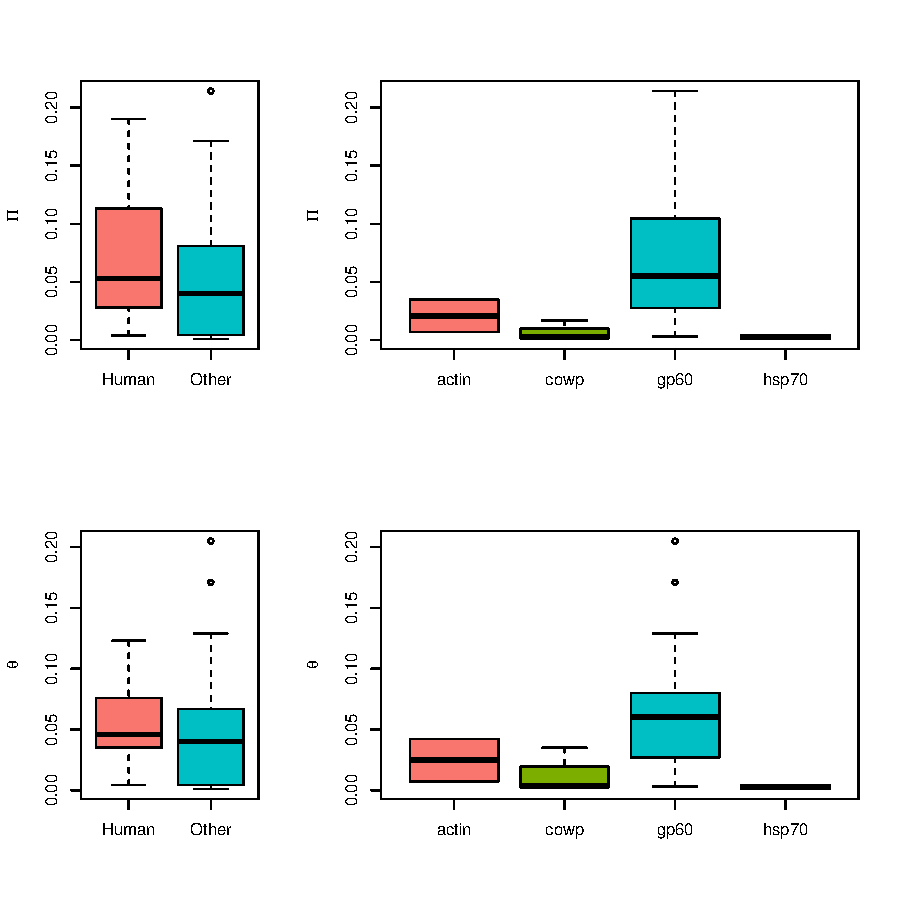
\includegraphics{Fig-test3}
\caption{All data}
\label{fig:w}
\end{figure}

\begin{figure}
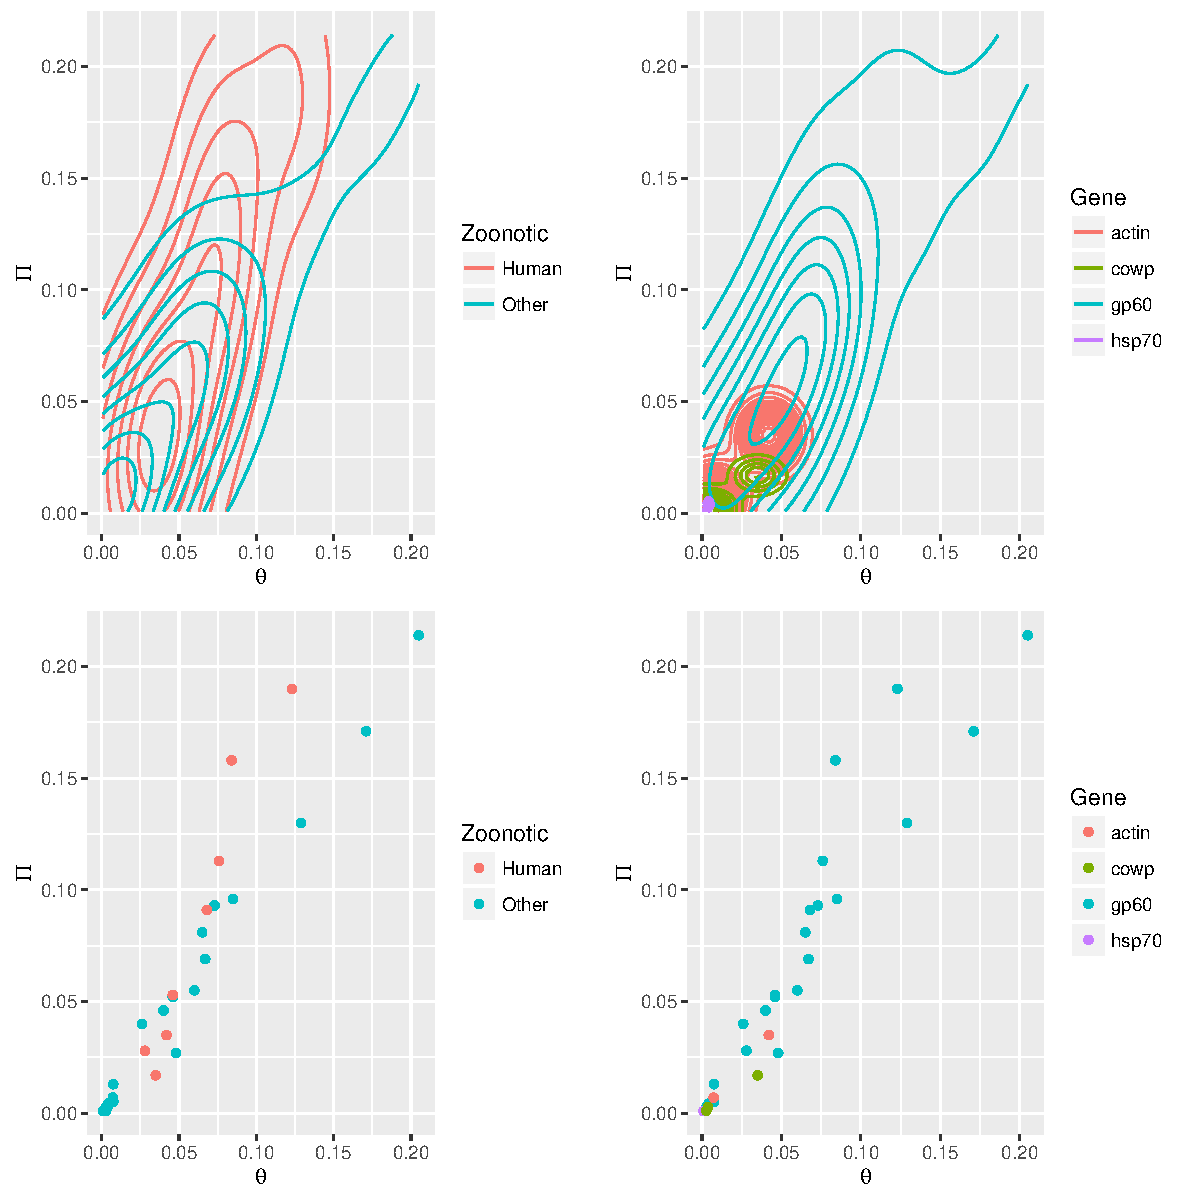
\includegraphics{Fig-test4}
\caption{All data diversity density}
\label{fig:x}
\end{figure}

%-------------------------------------------
\section{Zoonotic - gp60 data}
%--------------------------------------------

  
\begin{Schunk}
\begin{Sinput}
> fit <- manova(cbind(Species,Pi,Theta) ~ Zoonotic, data = newdata)
> summary(fit, test="Pillai")
\end{Sinput}
\begin{Soutput}
          Df  Pillai approx F num Df den Df   Pr(>F)   
Zoonotic   1 0.44224   5.0216      3     19 0.009911 **
Residuals 21                                           
---
Signif. codes:  0 '***' 0.001 '**' 0.01 '*' 0.05 '.' 0.1 ' ' 1
\end{Soutput}
\begin{Sinput}
> summary.aov(fit)
\end{Sinput}
\begin{Soutput}
 Response Species :
            Df Sum Sq Mean Sq F value Pr(>F)
Zoonotic     1  0.096 0.09591  0.0392  0.845
Residuals   21 51.382 2.44678               

 Response Pi :
            Df   Sum Sq   Mean Sq F value Pr(>F)
Zoonotic     1 0.007304 0.0073038  1.9459 0.1776
Residuals   21 0.078821 0.0037534               

 Response Theta :
            Df   Sum Sq    Mean Sq F value Pr(>F)
Zoonotic     1 0.000406 0.00040604  0.1393 0.7127
Residuals   21 0.061203 0.00291443               
\end{Soutput}
\end{Schunk}

\begin{figure}
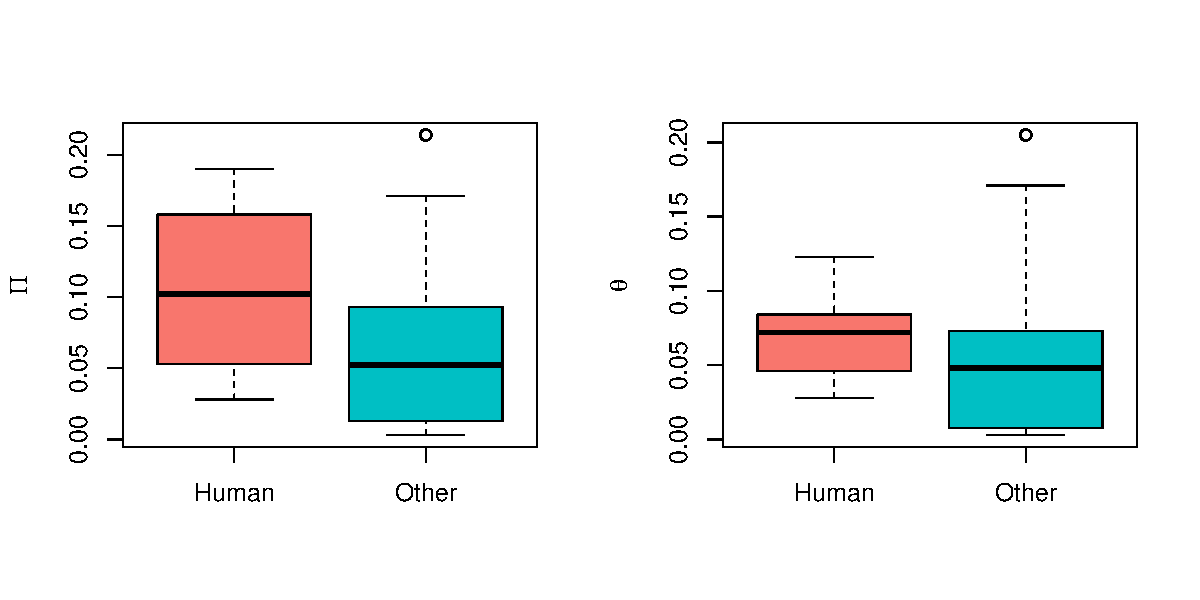
\includegraphics{Fig-test7}
\caption{gp60 diversity}
\label{fig:y}
\end{figure}

\begin{figure}
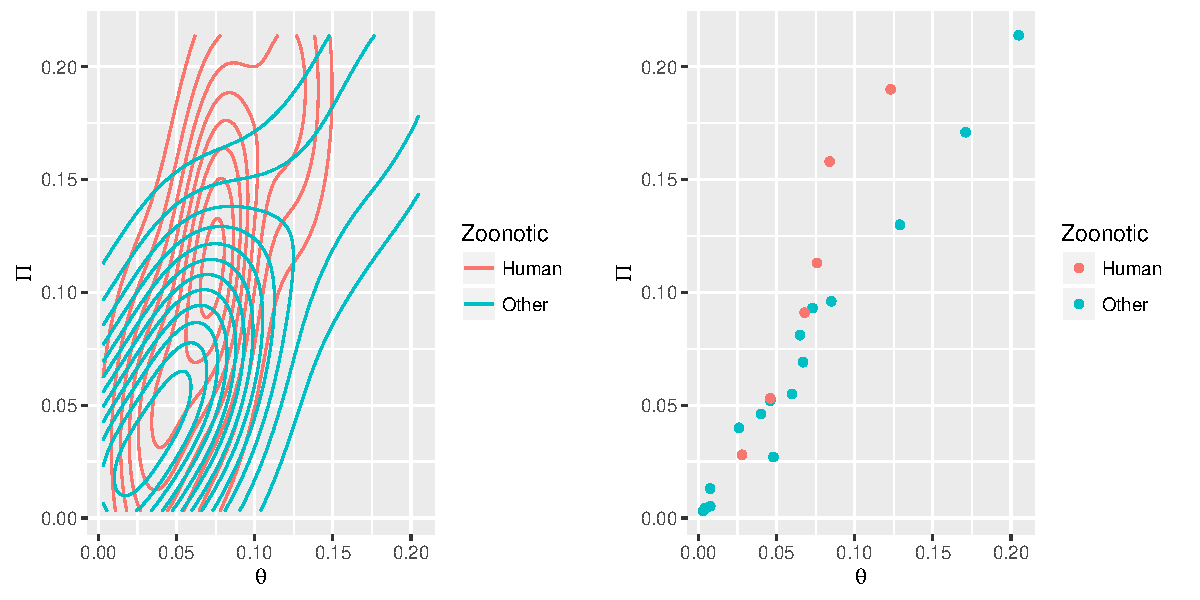
\includegraphics{Fig-test8}
\caption{gp60 diversity density}
\label{fig:z}
\end{figure}

\end{document}
